Sei \(\mathcal{M}^n\) eine kompakte, topologische Mannigfaltigkeit. Ist diese geschlossen, ist sie genau dann orientierbar, wenn \(H_n(\mathcal{M})\cong\mathbb{Z}\) gilt. Ist sie berandet, muss \(H_n(\mathcal{M},\partial\mathcal{M})\cong\mathbb{Z}\) gelten. Eine Wahl eines Erzeugers dieser Gruppen korrespondiert mit der Wahl einer Orientierung von \(\mathcal{M}\), hei\ss e \textbf{Fundamentalklasse} von \(\mathcal{M}\) und wird gelegentlich unter leichtem Notationsmissbrauch mit \(\eqcl{\mathcal{M}}\) bezeichnet. Ist \(\mathcal{M}\) nicht zusammenh\"angend, sei eine Orientierung eine Wahl von Fundamentalklassen aller Komponenten. Im Folgenden werden alle Mannigfaltigkeit als orientierbar angenommen. Wenn \(\iota\colon\mathcal{M}\hookrightarrow\mathcal{W}\) eine Einbettung ist, kann \(\eqcl{\mathcal{M}}\) als Element von \(H_n(\mathcal{W})\) aufgefasst werden. Schreibe f\"ur die inkludierte Homologieklasse
\[\eqcl{\mathcal{M}\mathrel{|}\mathcal{W}}:=\iota_*\eqcl{\mathcal{M}}\in H_n(\mathcal{W})\,.\]
Ist \(\mathcal{M}\) geschlossen, sagt die \textbf{Poincar\'e-Dualit\"at} nun gerade aus, dass der Homomorphismus 
\[H^k(\mathcal{M})\to H_{n-k}(\mathcal{M}),\,p\mapsto p\frown\eqcl{\mathcal{M}}\]
ein Isomorphismus ist (\cite{hatcher2002algebraic} Satz 3.30). Ist der Rand nicht leer, nimmt diese Isomorphie die Formen
\[H^k(\mathcal{M})\mathop{\cong}H_{n-k}(\mathcal{M},\partial\mathcal{M})\quad\text{und}\quad H^k(\mathcal{M},\partial\mathcal{M})\mathop{\cong}H_{n-k}(\mathcal{M})\]
an. Im Folgenden sei das duale Element von \(x\) auch durch \(x^*\) gekennzeichnet. Ist \(\mathcal{W}^n\) ein Kobordismus mit \(\partial\mathcal{W}\cong\partial_-\mathcal{W}\sqcup\partial_+\mathcal{W}\). Dann gilt die \textbf{Lefschetz-Dualit\"at}, also ist 
\[H^k(\mathcal{W},\partial_-\mathcal{W})\to H_{n-k}(\mathcal{W},\partial_+\mathcal{W}),\,\sigma\mapsto\sigma\frown\eqcl{\mathcal{W}}\,.\]
ist ein Isomorphismus (\cite{hatcher2002algebraic} Satz 3.43). Die langen exakten Folgen der Homomologie und der Kohomologie sind dabei durch folgendes bis auf Vorzeichen kommutative Diagramm verbunden (\cite{dold1980lectures} Abschnitt VIII Satz 9.1), in welchem \(i+j=n\) gelte.
\begin{equation}\label{diag:poin_exact}
    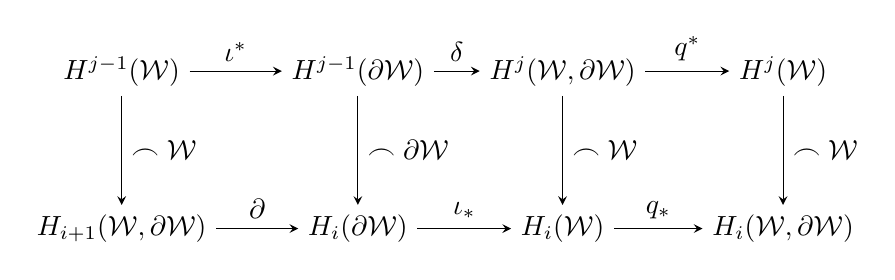
\begin{tikzpicture}[baseline=(current  bounding  box.center)]
        \draw 
            (0, 0) node (A) {\(H_{i+1}(\mathcal{W},\partial\mathcal{W})\)}
            (3, 0) node (B) {\(H_i(\partial\mathcal{W})\)}
            (5.6, 0) node (C) {\(H_i(\mathcal{W})\)}
            (8.4, 0) node (D) {\(H_i(\mathcal{W},\partial\mathcal{W})\)}
            (0, 2) node (E) {\(H^{j-1}(\mathcal{W})\)}
            (3, 2) node (F) {\(H^{j-1}(\partial\mathcal{W})\)}
            (5.6, 2) node (G) {\(H^j(\mathcal{W},\partial\mathcal{W})\)}
            (8.4, 2) node (H) {\(H^j(\mathcal{W})\)}
            (A) edge [-stealth] node [above] {\(\partial\)} (B)
            (B) edge [-stealth] node [above] {\(\iota_*\)} (C)
            (C) edge [-stealth] node [above] {\(q_*\)} (D)
            (E) edge [-stealth] node [above] {\(\iota^*\)} (F)
            (F) edge [-stealth] node [above] {\(\delta\)} (G)
            (G) edge [-stealth] node [above] {\(q^*\)} (H)
            (E) edge [-stealth] node [right] {\(\frown\eqcl{\mathcal{W}}\)} (A)
            (F) edge [-stealth] node [right] {\(\frown\eqcl{\partial\mathcal{W}}\)} (B)
            (G) edge [-stealth] node [right] {\(\frown\eqcl{\mathcal{W}}\)} (C)
            (H) edge [-stealth] node [right] {\(\frown\eqcl{\mathcal{W}}\)} (D)
            ;
    \end{tikzpicture}
\end{equation}